\documentclass[a4paper]{article}
\usepackage{amssymb}
\usepackage{array}
\usepackage{amsmath}
\usepackage[affil-it]{authblk}
\usepackage[backend=bibtex,style=numeric]{biblatex}
\usepackage{graphicx}
\usepackage{geometry}
\geometry{margin=1.5cm, vmargin={0pt,1cm}}
\setlength{\topmargin}{-1cm}
\setlength{\paperheight}{29.7cm}
\setlength{\textheight}{25.3cm}

\addbibresource{citation.bib}

\begin{document}
% =================================================
\title{Numerical Analysis homework \# 3}

\author{Chen Shuo 12231064
  \thanks{Email address: \texttt{shuo\_chen@zju.edu.cn}}}
\affil{(Electronic Science and Technology), Zhejiang University }


\date{Submitted time: \today}

\maketitle
% ============================================
\section*{I}
According to the problem, $s \in \mathcal{C}^k[0,2]$, i.e. $s(1^-) = s(1^+)$,$s'(1^-) = s'(1^+)$ and $s''(1^-) = s''(1^+)$. Assume that $p(x) = ax^3+bx^2+cx+d$, with $s(0)=p(0)=0$, then:

\begin{align*}
  d &= 0 \\
a+b+c+d &= 1 \\
3a+2b+c &= -3 \\
6a+2b &= 6
\end{align*}

Solve the equations above and get $a = 7$, $b = -18$, $c=12$, $d = 0$, then $p(x)=7x^3-18x^2+12x$. $s''(0) = p''(0) = -36$ and $s(x)$ is not a natural cubic spline.

\section*{II}
\subsection*{II-a}
$x_1, x_2, \cdots, x_n$ divide [a,b] into $n-1$ parts, each part $[x_i,x_{i+1}]$ with a polynomial $s_i$, $n-1$ polynomials in total. Due to $s \in \mathbb{S}_2^1$, which means $s_i \in \mathbb{P}_2$ and their derivates should be continuous.

To determine a quadratic polynomial, we need 3 independent equations, so there would be $3(n-1)$ independent equations needed in total. Now consider what we have: Firstly for each interval $[x_i,x_{i+1}]$, function values of two endpoints are 
known, so we get $2(n-1)$ equations. In addition, to be 1-order continuous on $[a,b]$, derivates should be continuous at $x_2,\cdots,x_{n-1}$, therefore another $n-2$ equations.

In total we get $2(n-1)+n-2=3n-4$ equations, so an additional condition is still needed in order to determine $s$ uniquely.

\subsection*{II-b}
$p_i \in \mathbb{P}_2$, assume that $p_i = ax^2+bx+c$. According to the problem, $p(x_i) = s(x_i) = f_i$, $p(x_{i+1}) = s(x_{i+1}) = f_{i+1}$, $p'(x_i) = s'(x_i) = m_i$, then:
\begin{align*}
a x_i^2 + b x_i + c &= f_i \\
a x_{i+1}^2 + b x_{i+1} + c &= f_{i+1} \\
2a x_i + b = m_i
\end{align*}
Solve the equations above and get:
\begin{align*}
a &= \frac{f_{i+1}-f_i}{(x_{i+1}-x_i)^2} - \frac{m_i}{x_{i+1}-x_i} \\
b &= \frac{x_{i+1}+x_i}{x_{i+1}-x_i}m_i - \frac{2x_i(f_{i+1}-f_i)}{(x_{i+1}-x_i)^2} \\
c &= f_i + \frac{x_i^2 (f_{i+1}-f_i)}{(x_{i+1}-x_i)^2} - \frac{m_i x_i x_{i+1}}{x_{i+1} - x_i}
\end{align*}
Therefore, $p_i(x) = (\dfrac{f_{i+1}-f_i}{(x_{i+1}-x_i)^2} - \dfrac{m_i}{x_{i+1}-x_i})x^2 + (\dfrac{x_{i+1}+x_i}{x_{i+1}-x_i}m_i - \dfrac{2x_i(f_{i+1}-f_i)}{(x_{i+1}-x_i)^2})x +f_i + \dfrac{x_i^2 (f_{i+1}-f_i)}{(x_{i+1}-x_i)^2} - \dfrac{m_i x_i x_{i+1}}{x_{i+1} - x_i}$

\subsection*{II-c}
According to II-b, we can get $p_1(x)$ with $m_1$, $f_1$ and $f_2$. Then we can calculate $m_2 = s'(x_2) = p_1^{'}(x_2)$. By using $m_2$, $f_2$ and $f_3$ we can get $p_2(x)$ then calculate $m_3$.

Repeat this process $n-2$ times and we get $m_2,m_3,\cdots, m_{n-1}$.

\section*{III}
$s(x)$ is a natural cubic spline so $s(x) \in \mathbb{S}_3^2$, which means $s_1(0) = s_2(0)$, $s_1^{'}(0) = s_2^{'}(0)$ and $s_1^{''}(0) = s_2^{''}(0)$. Assume that $s_2(x) = a_3x^3+a_2x^2+a_1x+a_0$:
\begin{align*}
  a_0 &= 1+c \\
  a_1 &= 3c \\
  2a_2 &= 6c
\end{align*}
In addition, $s_2^{''}(1) = 0$ because $s(x)$ is a natural cubic spline, i.e. $6a_3+2a_2=0$.

Therefore, $s_2(x) = -cx^3+3cx^2+3cx+c+1$.

If one wants $s(1) = 6c+1 = -1$ ,then $c = -\frac{1}{3}$.

\section*{IV}
\subsection*{IV-a}
Denote the spline as $s(x)$:
$$
s(x) = \left\{
\begin{aligned}
& s_1(x), x\in [-1,0] \\
& s_2(x), x\in [0,1]
\end{aligned}
\right.
$$
Assume that $s_1(x) = a_3x^3 + a_2x^2 + a_1x + a_0$ and $s_2(x) = b_3x^3 + b_2x^2 + b_1x + b_0$.
$s(x) \in \mathbb{S}_3^2$, and $s(x)$ is a natural cubic spline, then:
\begin{align*}
s_1(-1) &= f(-1) \\
s_1(0) &= f(0) \\
s_1^{'}(0) &= s_2^{'}(0) \\
s_1^{''}(0) &= s_2^{''}(0) \\
s_2(0) &= f(0) \\
s_2(1) &= f(1) \\
s_1^{''}(-1) &= 0 \\
s_2^{''}(1) &= 0
\end{align*}
Solve the equations above and get $s_1(x) = -\dfrac{1}{2}x^3 - \dfrac{3}{2}x^2 + 1$, $s_2(x) = \dfrac{1}{2}x^3 - \dfrac{3}{2}x^2 + 1$.

\subsection*{IV-b}
$f(x) = cos(\frac{\pi}{2}x)$, then $f(-1) = 0$, $f(0) = 1$, $f(1) = 0$. $g(x)$ is a quadratic polynomial and assume that $g(x) = ax^2+bx+c$. With the function value at -1, 0, 1 we can get 
$g(x) = -x^2+1$. Now calculate bending energy of three functions:
\begin{align*}
\int_{-1}^{1}[g''(x)]^2dx &= \int_{-1}^{1}(-2)^2dx \\
&= 8 \\
\int_{-1}^{1}[f''(x)]^2dx &= \int_{-1}^{1}[-\frac{\pi^2}{4}\cos(\frac{\pi}{2}x)]^2dx \\
&= \frac{\pi^4}{16}\\
\int_{-1}^{1}[s''(x)]^2dx &= \int_{-1}^0[s_1''(x)]^2dx + \int_{0}^1[s_2''(x)]^2dx \\
&= \int_{-1}^0[-3x-3]^2dx + \int_{0}^1[3x-3]^2dx \\
&= 6
\end{align*}
Therefore, $s(x)$ has the minimum bending energy of three functions.

\section*{V}
\subsection*{V-a}
According to the book:
$$
B_i^1(x) = \left\{
\begin{aligned}
&\frac{x-t_{i-1}}{t_{i}-t_{i-1}}, x \in (t_{i-1},t_i] \\
&\frac{t_{i+1}-x}{t_{i+1}-t_{i}}, x \in (t_{i},t_{i+1}] \\
&0, otherwise
\end{aligned}
\right.
$$
$B_i^2(x) = \dfrac{x-t_{i-1}}{t_{i+1}-t_{i-1}}B_i^1(x) + \dfrac{t_{i+2}-x}{t_{i+2}-t_{i}}B_{i+1}^1(x)$, then:
$$
B_i^2(x) = \left\{
\begin{aligned}
&\frac{(x-t_{i-1})^2}{(t_{i}-t_{i-1})(t_{i+1}-t_{i-1})}, x \in (t_{i-1},t_i] \\
&\frac{(x-t_{i-1})(t_{i+1}-x)}{(t_{i+1}-t_{i})(t_{i+1}-t_{i-1})} + \frac{(x-t_{i})(t_{i+2}-x)}{(t_{i+1}-t_{i})(t_{i+2}-t_{i})}, x \in (t_i,t_{i+1}] \\
&\frac{(t_{i+2}-x)^2}{(t_{i+2}-t_{i+1})(t_{i+2}-t_{i})}, x \in (t_{i+1},t_{i+2}] \\
&0, otherwise
\end{aligned}
\right.
$$

\subsection*{V-b}
$$
\frac{d}{dx}B_i^2(x_i^{-}) = \left.\frac{2(x-t_{i-1})}{(t_{i}-t_{i-1})(t_{i+1}-t_{i-1})}\right|_{x=t_i} = \frac{2}{t_{i+1}-t_{i-1}}
$$
$$
\frac{d}{dx}B_i^2(x_i^{+}) = \left.[\frac{-2x+t_{i-1}+t_{i+1}}{(t_{i+1}-t_{i})(t_{i+1}-t_{i-1})} + \frac{-2x+t_{i}+t_{i+2}}{(t_{i+1}-t_{i})(t_{i+2}-t_{i})}]\right|_{x=t_i} = \frac{2}{t_{i+1}-t_{i-1}}
$$
$$
\frac{d}{dx}B_i^2(x_{i+1}^{-}) = \left.[\frac{-2x+t_{i-1}+t_{i+1}}{(t_{i+1}-t_{i})(t_{i+1}-t_{i-1})} + \frac{-2x+t_{i}+t_{i+2}}{(t_{i+1}-t_{i})(t_{i+2}-t_{i})}]\right|_{x=t_{i+1}} = -\frac{2}{t_{i+2}-t_i}
$$
$$
\frac{d}{dx}B_i^2(x_{i+1}^{+}) = \left.\frac{2(x-t_{i+2})}{(t_{i+2}-t_{i+1})(t_{i+2}-t_{i})}\right|_{x=t_{i+1}} = -\frac{2}{t_{i+2}-t_i}
$$
Therefore, $\dfrac{d}{dx}B_i^2(x)$ is continuous at $t_i$ and $t_{i+1}$.

\subsection*{V-c}
According to V-b, $\dfrac{d}{dx}B_i^2(x) > 0$ if $x \in (t_{i-1},t_i]$, $\dfrac{d}{dx}B_i^2(x) < 0$ if $x \in (t_{i+1},t_{i+2})$.
In addition, $\dfrac{d}{dx}B_i^2(t_i) > 0$, $\dfrac{d}{dx}B_i^2(t_{i+1}) < 0$, $\dfrac{d}{dx}B_i^2(x)$ decreases monotonocally on $(t_i,t_{i+1})$ and it is continuous on $(t_i,t_{i+1})$, so there is only one 
$x^* \in (t_i,t_{i+1})$ which satisfies $\dfrac{d}{dx}B_i^2(x^*) = 0$.

Let $\dfrac{d}{dx}B_i^2(x^*) = 0$ and use the formula in V-b, we can get $x^* = \dfrac{t_{i+2}t_{i+1}-t_it_{i-1}}{t_{i+2}+t_{i+1}-t_i-t_{i-1}}$.

\subsection*{V-d}
According to V-c, $\dfrac{d}{dx}B_i^2(x)$ increases monotonocally on $(t_{i-1},x^*)$ and decreases monotonocally on $(x^*,t_{i+2})$.
$$
B_i^2(t_{i-1}) = 0
$$
$$
B_i^2(t_{i+2}) = 0
$$
$$
B_i^2(x^*) = \frac{(t_{i+2}-t_{i-1})(t_{i+1}-t_{i-1})}{(t_{i+2}+t_{i+1}-t_i-t_{i-1})^2}
+ \frac{(t_{i+2}-t_{i})(t_{i+2}-t_{i-1})}{(t_{i+2}+t_{i+1}-t_i-t_{i-1})^2}
= \frac{t_{i+2}-t_{i-1}}{t_{i+2}+t_{i+1}-t_i-t_{i-1}} < 1
$$
Therefore, $B_i^2(x) \in (0,1]$

\subsection*{V-e}
\begin{figure}[htbp]
  \centering
  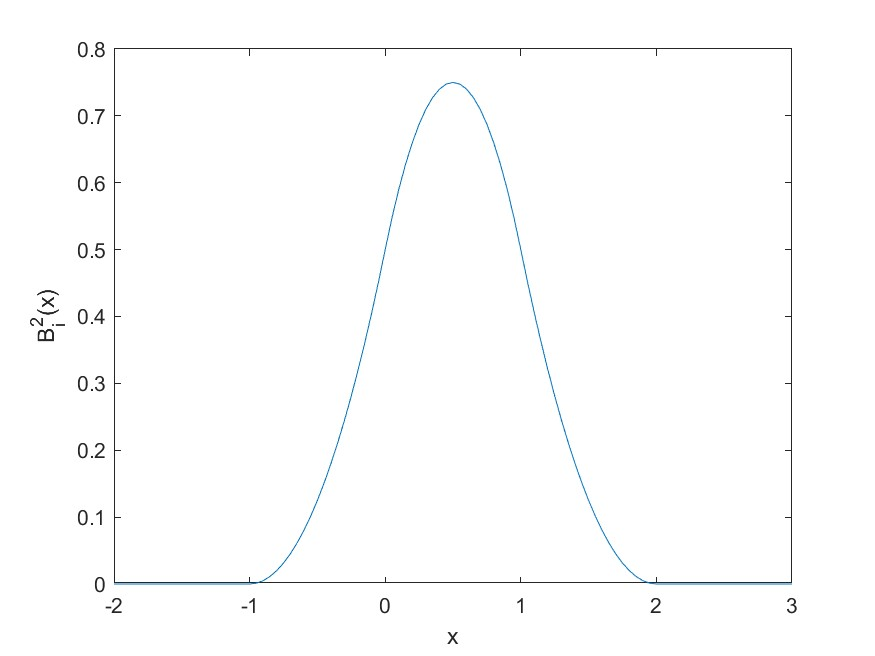
\includegraphics[width=0.6\textwidth]{fig/ProblemV-e.jpg}
  \caption{ProblemV-e}
  \label{fig:ProblemV-e}
\end{figure}

\section*{VI}
\begin{align*}
& (t_{i+2} - t_{i-1})[t_{i-1}, t_i, t_{i+1}, t_{i+2}](t - x)_+^2 \\
&= \frac{1}{t_{i+2} - t_i}(\frac{(t_{i+2} - x)_+^2 - (t_{i+1} - x)_+^2}{t_{i+2} - t_{i+1}} - \frac{(t_{i+1} - x)_+^2 - (t_{i} - x)_+^2}{t_{i+1} - t_{i}}) \\
&- \frac{1}{t_{i+1} - t_{i-1}}(\frac{(t_{i+1} - x)_+^2 - (t_{i} - x)_+^2}{t_{i+1} - t_{i}} - \frac{(t_{i} - x)_+^2 - (t_{i-1} - x)_+^2}{t_{i} - t_{i-1}})
\end{align*}
Let $\alpha(x) = \dfrac{1}{t_{i+2} - t_i}(\dfrac{(t_{i+2} - x)_+^2 - (t_{i+1} - x)_+^2}{t_{i+2} - t_{i+1}} - \dfrac{(t_{i+1} - x)_+^2 - (t_{i} - x)_+^2}{t_{i+1} - t_{i}})$ and 
$\beta(x) = \dfrac{1}{t_{i+1} - t_{i-1}}(\dfrac{(t_{i+1} - x)_+^2 - (t_{i} - x)_+^2}{t_{i+1} - t_{i}} - \dfrac{(t_{i} - x)_+^2 - (t_{i-1} - x)_+^2}{t_{i} - t_{i-1}})$.

$$
\alpha(x) = \left\{
\begin{aligned}
& 1, x\in (-\infty,t_i] \\
& \frac{1}{t_{i+2}-t_i}(t_{i+2}+t_{i+1}-2x-\frac{(t_{i+1}-x)^2}{t_{i+1}-t_i}) ,x \in (t_i,t_{i+1}] \\
& \frac{1}{t_{i+2}-t_i}\cdot\frac{(t_{i+2}-x)^2}{t_{i+2}-t_{i+1}}, x \in (t_{i+1},t_{i+2}] \\
& 0, x \in (t_{i+2},+\infty)
\end{aligned}
\right.
$$
$$
\beta(x) = \left\{
\begin{aligned}
& 1, x\in (-\infty,t_{i-1}] \\
& \frac{1}{t_{i+1}-t_{i-1}}(t_{i+1}+t_{i}-2x-\frac{(t_{i}-x)^2}{t_{i}-t_{i-1}}) ,x \in (t_{i-1},t_{i}] \\
& \frac{1}{t_{i+1}-t_{i-1}}\cdot\frac{(t_{i+1}-x)^2}{t_{i+1}-t_{i}}, x \in (t_{i},t_{i+1}] \\
& 0, x \in (t_{i+1},+\infty)
\end{aligned}
\right.
$$
Therefore, it can be divided into several cases:
\begin{itemize}
  \item $x \in (-\infty,t_{i-1}]$, $\alpha(x) - \beta(x) = 1 - 1 = 0$.
  \item $x \in (t_{i-1},t_i]$, $\alpha(x) - \beta(x) = 1 - \dfrac{1}{t_{i+1}-t_{i-1}}(t_{i+1}+t_{i}-2x-\dfrac{(t_{i}-x)^2}{t_{i}-t_{i-1}})
= \dfrac{(x-t_{i-1})^2}{(t_i-t_{i-1})(t_{i+1}-t_{i-1})}$.
  \item $x \in (t_{i},t_{i+1}]$, $\alpha(x) - \beta(x) = \dfrac{1}{t_{i+2}-t_i}(t_{i+2}+t_{i+1}-2x-\dfrac{(t_{i+1}-x)^2}{t_{i+1}-t_i})
- \dfrac{1}{t_{i+1}-t_{i-1}}\cdot\dfrac{(t_{i+1}-x)^2}{t_{i+1}-t_{i}} = \dfrac{(x-t_{i-1})(t_{i+1}-x)}{(t_{i+1}-t_{i})(t_{i+1}-t_{i-1})} + \dfrac{(x-t_{i})(t_{i+2}-x)}{(t_{i+1}-t_{i})(t_{i+2}-t_{i})}$
  \item $x \in (t_{i+1},t_{i+2}]$, $\alpha(x) - \beta(x) = \dfrac{(t_{i+2}-x)^2}{(t_{i+2}-t_{i+1})(t_{i+2}-t_{i})}$
  \item $x \in (t_{i+2},+\infty)$, $\alpha(x) - \beta(x) = 0$.
\end{itemize}
Therefore, 
$$
\alpha(x) - \beta(x) = \left\{
\begin{aligned}
& 0, x \in (-\infty,t_{i-1}] \\
& \dfrac{(x-t_{i-1})^2}{(t_i-t_{i-1})(t_{i+1}-t_{i-1})}, x \in (t_{i-1},t_i] \\
& \dfrac{(x-t_{i-1})(t_{i+1}-x)}{(t_{i+1}-t_{i})(t_{i+1}-t_{i-1})} + \dfrac{(x-t_{i})(t_{i+2}-x)}{(t_{i+1}-t_{i})(t_{i+2}-t_{i})} ,x \in (t_{i},t_{i+1}] \\
& \frac{(t_{i+2}-x)^2}{(t_{i+2}-t_{i+1})(t_{i+2}-t_{i})}, x \in (t_{i+1},t_{i+2}] \\
& 0, x \in (t_{i+2},+\infty)
\end{aligned}
\right.
$$
Compared to the formula in V-a, and get the conclusion that $B_i^2(x) = (t_{i+2} - t_{i-1})[t_{i-1}, t_i, t_{i+1}, t_{i+2}](t - x)_+^2$.

\section*{VII}
By Theorem 3.34 we know $\dfrac{d}{dx}B_i^n(x) = \dfrac{nB_i^{n-1}(x)}{t_{i+n-1}-t_{i-1}} - \dfrac{nB_{i+1}^{n-1}(x)}{t_{i+n}-t_i}$.

Take the integral of two sides from $t_{i-1}$ to $t_{i+n}$:
$$
\int_{t_{i-1}}^{t_{i+n}}\frac{d}{dx}B_i^n(x)dx = B_i^n(x) \bigg|_{t_{i-1}}^{t_{i+n}} = 0
$$
$$
\int_{t_{i-1}}^{t_{i+n}}(\dfrac{nB_i^{n-1}(x)}{t_{i+n-1}-t_{i-1}} - \dfrac{nB_{i+1}^{n-1}(x)}{t_{i+n}-t_i})dx
= \dfrac{n}{t_{i+n-1}-t_{i-1}}\int_{t_{i-1}}^{t_{i+n-1}}B_i^{n-1}(x)dx - \dfrac{n}{t_{i+n}-t_{i}}\int_{t_{i}}^{t_{i+n}}B_{i+1}^{n-1}(x)dx
$$
Hence $\displaystyle\dfrac{n}{t_{i+n-1}-t_{i-1}}\int_{t_{i-1}}^{t_{i+n-1}}B_i^{n-1}(x) - \dfrac{n}{t_{i+n}-t_{i}}\int_{t_{i}}^{t_{i+n}}B_{i+1}^{n-1}(x) = 0$ 

i.e.:
$\dfrac{1}{t_{i+n-1}-t_{i-1}}\displaystyle\int_{t_{i-1}}^{t_{i+n-1}}B_i^{n-1}(x) = \dfrac{1}{t_{i+n}-t_{i}}\int_{t_{i}}^{t_{i+n}}B_{i+1}^{n-1}(x)$

Therefore, the scaled integral of $B_i^n(x)$ over its support is independent of its index.

\section*{VIII}
\subsection*{VIII-a}
Calculate $[x_i,x_{i+1},x_{i+2}]x^4$ with the table of divided difference:
$$
\begin{array}{c|c c c c c c}
  x_i & x_i^4 \\
  x_{i+1} & x_{i+1}^4 & x_{i+1}^3 + x_{i+1}^2x_i + x_{i+1}x_i^2 + x_i^3 \\
  x_{i+2} & x_{i+2}^4 & x_{i+2}^3 + x_{i+2}^2x_{i+1} + x_{i+2}x_{i+1}^2 + x_{i+1}^3 & x_i^2 + x_ix_{i+1} + x_ix_{i+2} + x_{i+1}^2 +x_{i+1}x_{i+2} + x_{i+2}^2 \\
\end{array}
$$
According to the definition of complete symmetric polynomials:
\begin{align*}
\tau_2(x_i,x_{i+1},x_{i+2}) &= \sum\limits_{i\leq i_1 \leq i_2 \leq i+2} x_{i_1}x_{i_2} \\
&= x_i^2 + x_ix_{i+1} + x_ix_{i+2} + x_{i+1}^2 +x_{i+1}x_{i+2} + x_{i+2}^2
\end{align*}

Compare two results and they are same.

\subsection*{VIII-b}
Recursive relations of complete symmetric polynomials says that:
$$
\tau_{k+1}(x_1,\cdots,x_n,x_{n+1})
= \tau_{k+1}(x_1,\cdots,x_n) + x_{n+1}\tau_k(x_1,\cdots,x_n,x_{n+1})
$$
Then we have:
\begin{align*}
  (x_{n+1} - x_1) \tau_k (x_1, \dots, x_n, x_{n+1}) 
  &= \tau_{k+1}(x_1, \dots, x_n, x_{n+1}) - \tau_{k+1}(x_1, \dots, x_n) \\
  &\quad - x_1 \tau_k(x_1, \dots, x_n, x_{n+1}) \\
  &= \tau_{k+1}(x_2, \dots, x_n, x_{n+1}) + x_1 \tau_k(x_1, \dots, x_n, x_{n+1}) \\
  &\quad - \tau_{k+1}(x_1, \dots, x_n) - x_1 \tau_k(x_1, \dots, x_n, x_{n+1}) \\
  &= \tau_{k+1}(x_2, \dots, x_n, x_{n+1}) - \tau_{k+1}(x_1, \dots, x_n).
\end{align*}
For $n=0$, $\tau_m(x_i) = x_i^m = [x_i]x^m$.

Suppose that $\forall m \in \mathbb{N}^+$, $\forall i \in \mathbb{N}$, $\forall n = 0,1,\cdots,m$,
$\tau_{m-n}(x_i,\cdots,x_{i+n}) = [x_i,\cdots,x_{i+n}]x^m$ holds for a non-negative integer $n<m$, then:
\begin{align*}
  \tau_{m-n-1}(x_i, \dots, x_{i+n+1}) 
  &= \frac{\tau_{m-n}(x_{i+1}, \dots, x_{i+n+1}) - \tau_{m-n}(x_i, \dots, x_{i+n})}{x_{i+n+1} - x_i} \\
  &= \frac{[x_{i+1}, \dots, x_{i+n+1}] x^m - [x_i, \dots, x_{i+n}] x^m}{x_{i+n+1} - x_i} \\
  &= [x_i, \dots, x_{i+n+1}] x^m.
\end{align*}
Therefore it holds for the case $n+1$, by induction this proof is done.

\end{document}


